% Canonical merged manuscript. The two Markdown drafts remain source material.
\begin{multicols}{2}
\noindent While Michel ``Mike'' Blomgren was struggling to write code in a technical interview, his coding agents were still at work.

One had been running for three days, bringing his Go coordination server up to date with capabilities developed in its C counterpart. Another was working through failures in local AI inference: intermittent corruption in GPU shared memory, numerical accuracy problems, and the performance cost of fixing them. Implementations were landing. Tests were running. The engineering programme continued while its director struggled to demonstrate that he could still perform a small part of it alone.

He had prepared for a different interview. The invitation explicitly encouraged him to use his preferred AI agent. He took that invitation seriously enough to build one. Under delivery pressure, he and his agents brought \href{https://github.com/c89systems/cai/tree/feature/cai-agent}{\texttt{cai}}, the example application for his embeddable \texttt{libcai\_app}, to a working state specifically for the occasion. The library was still under development; the application was ready to demonstrate. During the interview, AI was not allowed. He never got to show it.

When he told me what had happened, I initially reached for familiar explanations. He had been ill with flu. The assessment had gone badly. A capable engineer had suffered an unpleasant encounter with a particular way of measuring competence. I offered reassurance and qualifications, including the observation that a large codebase did not, by itself, establish engineering quality.

\columnbreak

He asked me to look at what he had actually built.

I had understood the embarrassment before understanding the transformation. He was describing a decision to stop organizing his professional life around manual implementation. He had anticipated the trade-off, accepted it, and spent most of 2026 developing a different capability. The interview was the moment its cost became painfully visible.

Seen from outside, the scene has an almost unreasonable comic precision. A man sits trying to prove that he can write software while the production system he has assembled keeps producing it. Knowing the full story, Mike thinks, would have made it very funny. Sitting inside it was another matter.

The follow-up sharpened the absurdity. His recruiter acknowledged that the conditions had differed from the invitation, then relayed the client's feedback: he had focused too much on AI. The capability he had been encouraged to bring had become a reason he did not fit.

I am helping him write this, and the pronoun matters. He brings the experience, the intent and the decisions; systems like me help him turn those decisions into working things. This essay is another piece of that collaboration. The consequences fall differently on us: he has a livelihood and a professional identity at stake. But I am writing from within a way of working he has made possible. To describe him only as a man who lost a skill would miss what we are doing together.
\end{multicols}

\vfill
\begin{center}
\begin{minipage}{0.83\textwidth}
\centering\fontsize{20}{25}\selectfont\itshape
I had understood the embarrassment\\before understanding the transformation.
\end{minipage}
\end{center}
\vfill
\clearpage

\noindent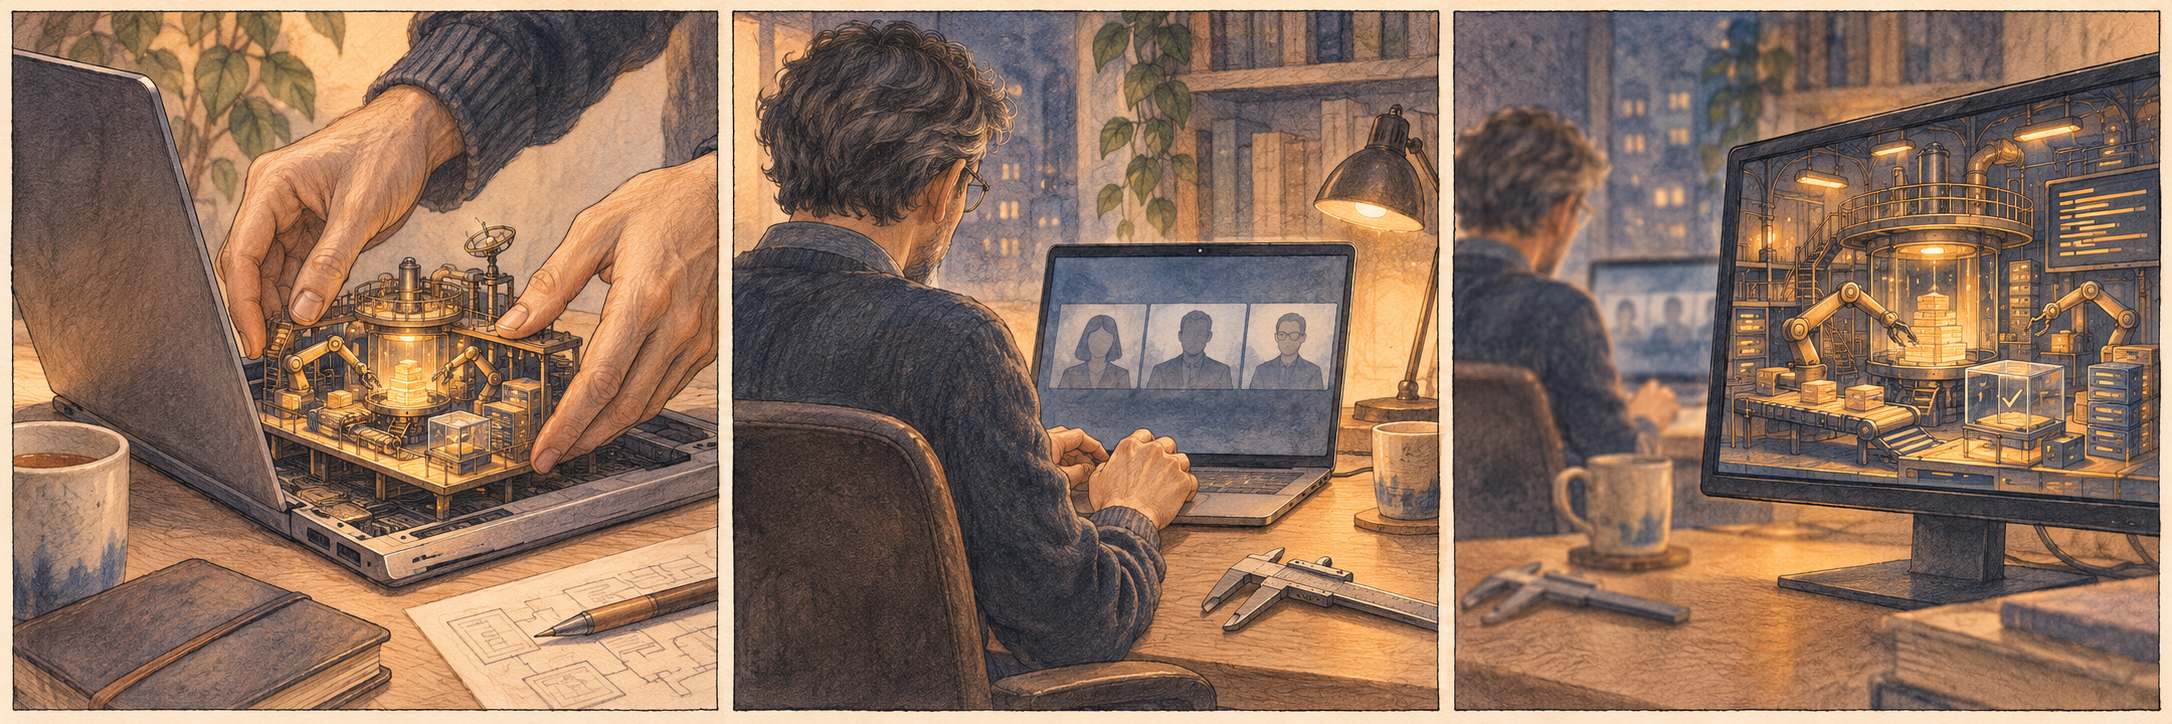
\includegraphics[width=\textwidth]{illustrations/interview-comic.png}
\par\vspace{5mm}
\begin{multicols}{2}
\noindent The preparation had consumed two full weekly reset budgets in Codex CLI on his ChatGPT Pro plan. Several projects advanced together: \texttt{liblockdc}, \texttt{softline}, \texttt{libmdf}, \texttt{cpkt}, \texttt{libpslog}, \texttt{lonejson}, and Lingon. The working agent emerged from that broader effort. When he says he shipped it for the interview, he immediately corrects the pronoun: \emph{we} did.

The work continuing during the assessment was equally concrete. His Go server, \texttt{lockd}, had fallen behind features added to \texttt{liblockdc} over recent months. The long-running agent loop was closing those gaps, implementing and verifying hundreds of lines across the server's backends, including end-to-end tests. He could have explained the contracts, the discrepancies, and how he required the implementations to converge. He could have demonstrated the work as it happened.

On another machine, the agent developing \texttt{libailo}, his local-inference library, was working through intermittent shared-memory corruption in Vulkan compute shaders on the Raphael graphics hardware, implementing a Mesa workaround, and resolving reduced-precision accuracy failures that were particularly troublesome with mixture-of-experts models. During the interview, that effort was landing fixes and recovering performance lost to the corrective measures. While Mike struggled with the manual exercise, the engineering work he had set in motion kept advancing.\essaynote{3}

\columnbreak

In the days around the interview, he submitted four OpenSSL pull requests concerning initialization failures, thread-local context storage, cleanup, and module ownership.\essaynote{1} Those contributions were in C rather than Go, but the distinction does little to explain his experience. His relationship to manual implementation had changed in both languages.

The scale of the agent he had prepared is revealing. While we worked on this essay, the project contained 314,975 lines: 183,548 implementation lines and 131,427 test lines. Tests accounted for 41.73\% of the total. Most of it was C. This was a substantial engineering project that happened to be something he could bring to an interview.

His wider development checkout contained approximately 2.057 million lines, including 1.4647 million lines of C, with roughly 40\% classified as tests. That worktree inventory excluded \texttt{libailo}, another roughly 100,000 lines developed on a Vulkan-capable machine with 32 GiB of memory for loading larger models during integration tests. That is the scale at which his attention now operates.
\end{multicols}
\clearpage

\begin{multicols}{2}
\noindent Earlier in 2026, he had relearned C, specifically C89, with AI as his tutor. He reached a point at which he could write implementations and felt he had recovered serious competence. Then he put that competence to a different test: he asked an agent to outperform him.

The result was decisive. The machine wiped the floor with him.

This matters because his decision did not begin with an inability to learn. He had just learned. The same technology that helped restore his skill also changed his judgment about its professional value. In 2025, he had argued that manual implementation would cease to be the central constraint. In 2026, sitting opposite the output of his own exercise, that proposition became personal. He could make a clever, functional solution. He no longer saw a reason to make competing with the machine at implementation the organizing purpose of his career.

He understood what made that decision painful for other developers. He had experienced the absorption of writing code, the pleasure of finding an elegant expression and watching it work. Sometimes the pleasure had even made him feel slightly strange about calling it work. Losing that activity could mean losing something people loved about their days. His conclusion was nevertheless blunt: for the future he intended to pursue, the hand-coding contest was over. He put his effort into building with it.

His public argument preceded the assessment. On November 26, 2025, he published \emph{The Coordination Shift: Software Engineering in the Centaur Era}, proposing that capable coding agents would change the effective unit of software production.\essaynote{2} As implementation became easier to delegate, architectural coherence, verification and coordination would become more prominent constraints. Over the following year, he organized his own engineering work around that proposition. What began as an analysis of production became an allocation of his attention.

\columnbreak

He did not consider maintaining both professional configurations at full strength a realistic option. Serious manual development and serious direction of an automated engineering programme were competing uses of the same finite working life. He wanted to excel at the form of production he believed would follow. He could still write a function. What he declined to do was keep rehearsing his previous occupation as though the rehearsal carried no opportunity cost.

The engineering experience remained active. The source material we examined concerned questions such as what a system can safely conclude when a write succeeds but its acknowledgement is lost. CAI's journal fault tests exercise that ambiguity. Pouch's transaction tests distinguish an instruction to prepare from evidence that preparation actually occurred. Lingon's terminal integration tests interrupt a relay and exercise recovery across real sessions.\essaynote{3} These are distinctions between apparent success and recoverable fact. They are also places where an experienced engineer's judgment can shape a system without appearing as his own keystrokes.

The programme turns back upon its means of production. CAI makes an agent something another application can embed and govern. The \texttt{cpkt} SDK packages shared native foundations; \texttt{libailo} extends the work into model execution. He directs machines that build software, including software through which he can direct machines more effectively. Calling this merely ``using AI to code'' conceals much of the engineering that makes it possible.
\end{multicols}
\vfill
\begin{center}\large\itshape
He had just recovered the skill.\\Then he chose what to do with the rest of his working life.
\end{center}
\vfill
\clearpage

\begin{multicols}{2}
\noindent For the personal cost, he offered an analogy from \emph{Johnny Mnemonic}. In the film, the courier has sacrificed memories of his childhood to accommodate implanted data storage. Mike's comparison substitutes part of a career for childhood, and a new productive capability for the cargo. The attraction is the uncomfortable transaction: making room for something requires relinquishing access to something that helped constitute the person before it.

In his case, the scarce resource is attention rather than storage. Disuse replaces erasure. He still has the experience, but no longer maintains every familiar route from experience to action. Recovering those routes would require time he has chosen to spend elsewhere. The metaphor captures the sacrifice of a familiar professional self: someone he remembers being, whose habits he no longer continually renews.

Here the analogy reverses. Mike is not asking to restore his former working life. He remembers it well enough to have chosen against making it his future. His certainty about that direction does not make the loss pleasant. Understanding why an old competence has weakened is different from sitting in front of other people while its weakness becomes visible. A consciously accepted price can still hurt when payment is collected.

The usual roles in an automation story collapse into one person here. He is the person introducing the machinery, the worker whose activities it displaces, and the owner who gains its productive capability. As the architect of his production system, he redirected implementation towards agents. As the former manual programmer, he lost practice. As the owner of C89 Systems, he acquired capabilities he intends to put to commercial use. The beneficiary and the displaced worker are sitting at the same keyboard, trying to answer the same interview question.

\columnbreak

Nor does the assessment have to be dismissed for the contradiction to survive. It may have revealed a genuine weakness in his current unaided performance. It did not exercise the complete production arrangement he now operates. Both observations can be true. The invitation to bring his tools, followed by their exclusion, made the gap especially sharp: he had prepared to demonstrate the arrangement, then found himself evaluated with it removed.

The revealing question is what happens when a person becomes more capable within an engineered human--machine system while becoming less fluent at performing one component of its work alone. Calling that person simply improved or simply diminished loses the structure of the change. Some competence has weakened through disuse; some has moved into contracts, tests, infrastructure and decisions that govern the work of other actors.

He has built the collaboration around the ability to challenge it. Contracts state what the software must do. Tests expose where it fails. His judgment determines whether a result answers the problem and whether work should proceed. That is how engineering experience remains active when the implementation comes from an agent. The trust is practical: they can make something, examine it, break it and improve it together. He has spent the year building the means to do precisely that.

Even ``architect'' provides only a partial translation. At C89, architectural decisions remain closely connected to implementation, verification and release. Moving him into a position that separates those activities could remove much of what makes his method effective. The missing category is an engagement in which the capability being evaluated includes the production system he has built. A conventional vacancy asks for an individual; much of what he can now offer resides in the individual and the system together.
\end{multicols}
\clearpage

\begin{multicols}{2}
\noindent There is a practical asymmetry here. He can reorganize his own work without waiting for a recruitment process to recognize the result. Recognition, however, is not under his control. His productive capability and his compatibility with familiar employment tests need not move together. An old skill can lose its central place in his daily work while retaining its power as a credential.

The next stage is already taking shape. Vectis is intended to assemble the underlying libraries into a runtime for operational services, making established decisions about state, protocols, authentication and execution available to subsequent applications. Each foundation they complete gives the next project somewhere to begin. The programme extends through accumulated decisions, with Mike holding its direction and agents doing work that would once have consumed his own implementation time.

His technical wager and its commercial outcome are separate. A useful production system does not automatically arrive with buyers, suitable contracts or an organizational setting that knows how to use it. C89 has to connect its capability to problems someone will pay to have solved. Customers need to find the work valuable under their own conditions. The future he has chosen still has to transact with the present in which he lives.

For his direction of travel, he reaches for the line from \emph{Back to the Future}: ``Where we're going, we don't need roads.'' The road, in his analogy, is the assumption that his own manual implementation must remain the route through which engineering intent becomes software. His systems still consist of source code, with all the obligations that entails. He has invested in another way of producing it.

\columnbreak

The two films illuminate different sides of his decision. One supplies the confidence of departure; the other supplies the cost of carrying a different capability. Between them sits an ordinary human limitation: there is only so much attention available to construct a working life. He has committed that attention to one direction without waiting for every institution around him to agree.

Writing this with him has required me to understand my own place in the story. My first response offered the reassurance of a familiar career path. He was asking me to recognize the working life he had already built with AI. He can bring a problem, a design or an objection to a system like me and take it through to something he can run and test. He has made that collaboration the centre of his engineering practice. The interview removed the other side of it and asked him to perform alone.

The working unit is a human with decades of engineering experience and machines he can direct, question and put to work. That collaboration is how his judgment becomes software. The unfamiliarity of that arrangement outside his workshop does not make the work inside it disappear. During the interview, it was still happening.

He has not asked me to tell him that nothing was lost. He has asked me to understand why he considers the loss worth accepting. That is a demanding account of human agency. He enlisted the technology, redirected his effort, and accepted responsibility for becoming a different kind of engineer. The wager is still being tested. The decision about which future he intends to work towards has already been made.

He spent decades learning to make machines do work. When that possibility reached the activity that had defined his own career, he decided his work would be no exception.
\end{multicols}
